\documentclass[10pt,journal,compsoc]{IEEEtran}

\usepackage{cite}
\usepackage{amsmath,amssymb,amsfonts}
\usepackage{algorithmic}
\usepackage{graphicx}
\usepackage{textcomp}
\usepackage{url}

% correct bad hyphenation here
\hyphenation{op-tical net-works semi-conduc-tor}
%\setcounter{biburllcpenalty}{7000}
%\setcounter{biburlucpenalty}{8000}
\def\UrlBreaks{\do\/\do-}
\begin{document}
%
% paper title
% Titles are generally capitalized except for words such as a, an, and, as,
% at, but, by, for, in, nor, of, on, or, the, to and up, which are usually
% not capitalized unless they are the first or last word of the title.
% Linebreaks \\ can be used within to get better formatting as desired.
% Do not put math or special symbols in the title.
	%\title{Bare Demo of IEEEtran.cls for\\ IEEE Computer Society Journals}
%
\title{Overtaking Uncertainty with Evolutionary TORCS controllers:
  Combining adaptive BLX-$\alpha$ Operator and Grand Prix Selection}

\author{Mohammed~Salem, Antonio~M.~Mora, Juan~J.~Merelo% <-this % stops a space
\IEEEcompsocitemizethanks{\IEEEcompsocthanksitem M. Salem was with the Department of Computer Sciences, University of Mascara, Algeria.\protect\\
% note need leading \protect in front of \\ to get a newline within \thanks as
% \\ is fragile and will error, could use \hfil\break instead.
E-mail: salem@univ-mascara.dz
\IEEEcompsocthanksitem A~M.~Mora was with the Department of Signal Theory, Telematics and Communications, ETSIIT-CITIC, University of Granada, Spain.\protect\\
Email: amorag@ugr.es
\IEEEcompsocthanksitem J~J.~Merelo was with the Department of Computer Architecture and Computer Technology. University of Granada, Spain.\protect\\
Email: jmerelo@geneura.ugr.es
}% <-this % stops an unwanted space
\thanks{Manuscript received December XX, 2019; revised XXXX, 2020.}}

% note the % following the last \IEEEmembership and also \thanks - 
% these prevent an unwanted space from occurring between the last author name
% and the end of the author line. i.e., if you had this:
% 
% \author{....lastname \thanks{...} \thanks{...} }
%                     ^------------^------------^----Do not want these spaces!
%
% a space would be appended to the last name and could cause every name on that
% line to be shifted left slightly. This is one of those "LaTeX things". For
% instance, "\textbf{A} \textbf{B}" will typeset as "A B" not "AB". To get
% "AB" then you have to do: "\textbf{A}\textbf{B}"
% \thanks is no different in this regard, so shield the last } of each \thanks
% that ends a line with a % and do not let a space in before the next \thanks.
% Spaces after \IEEEmembership other than the last one are OK (and needed) as
% you are supposed to have spaces between the names. For what it is worth,
% this is a minor point as most people would not even notice if the said evil
% space somehow managed to creep in.



% The paper headers
%\markboth{Journal of \LaTeX\ Class Files,~Vol.~14, No.~8, August~2015}%
%{Shell \MakeLowercase{\textit{et al.}}: Bare Demo of IEEEtran.cls for Computer Society Journals}
% The only time the second header will appear is for the odd numbered pages
% after the title page when using the twoside option.
% 
% *** Note that you probably will NOT want to include the author's ***
% *** name in the headers of peer review papers.                   ***
% You can use \ifCLASSOPTIONpeerreview for conditional compilation here if
% you desire.



\IEEEtitleabstractindextext{%
  \begin{abstract}
    Evolution is a powerful problem-solving technique, which has been
extensively used for designing racing car controllers. It presents a
series of challenges: it needs an evaluation function that is able to
separate the best controllers from the rest, and it needs a series of
operators that are able to explore many different possibilities in the
controller (solutions) search space. But racing scores are variable and also
depend on adversaries and the actual track features and conditions. 
% This uncertainty also means that it is much more important to maintain a  high diversity. 
% Antonio - this is also said below
This adds to the problem an uncertainty that the designer of the algorithms must address or, at least, take into consideration.
Thus, building on the experience drawn from our previous work, in this paper we evaluate two novel operators in an evolutionary algorithm designed to optimize a controller for TORCS simulator. First, a kind of fitnessless selection policy based on competition and called \textit{Grand Prix Selection} (GPS), which should be able to reduce uncertainty by using something more realistic than solo race scores to select individuals. However, uncertainty has the unintended side effect of increasing diversity,
%%Mohammed: U mean uncertainty increases the diversity?? if so, how it does?
% Antonio - It was written by JJ, I guess he meant that dealing with uncertainty must require to have a more diverse population... "of increasing"-> "of requiring to increase"??
 so we will also evaluate the diversity-increasing BLX-$alpha$ operator, with varying value of $\alpha$, in combination with them, 
% Antonio - what does "them" refer to? GPS?
and see its % their?
%Mohammed :  it!!!
effects on overall performance. In general, results
will show that these combined improvements establish a new level of
performance of evolved controllers, being able to beat, both standard
and previously evolved controllers, as well as a high-ranked
controller of TORCS competitions.
\end{abstract}

% Note that keywords are not normally used for peerreview papers.
\begin{IEEEkeywords}
Simulated Car Racing, TORCS, Fuzzy Controllers, Autonomous
controllers, Genetic Algorithms, Optimization, BLX-$\alpha$ Crossover,
Grand Prix Selection, Fitnessless, Uncertainty, Competitive fitness 
\end{IEEEkeywords}}

% make the title area
\maketitle


\IEEEdisplaynontitleabstractindextext
\IEEEpeerreviewmaketitle



\IEEEraisesectionheading{\section{Introduction}\label{sec:introduction}}

Driving a car is a problem in which you have to map inputs that
include data about the environment we are driving in as well as car
data, to the output: throttling and steering. Car controllers have to
be designed so that cars do not crash, and are able to run at a
reasonable speed \cite{Autodriv2006}. Additionally, in a racing car the controller has to be designed so that the car wins in as many races as possible.

There are so many variables in this problem, that eventually some of
them are decided using heuristic rules, while the rest are open to
optimization. For instance, deciding the type of controller is usually
done before the design process begin, and a single, parametrized one
is chosen; fixed rules as well as neural networks \cite{KIM201287} or fuzzy controllers \cite{PerezEvolvingFuzzy09} are often used. 
Additionally to that, training (or learning) \cite{Loiacono:2012:LEA:2212908.2212953} can be done during the
race, so that it can adapt itself to new, and not seen before,
scenarios and competitors, or it can be fixed by training the
controllers in advance. 

We have been using genetically-optimized fuzzy controllers in this line of work, with increasing success.
However, in a simulated and realistic racing car environment like the one we use, racing car scores are a
    statistical variable whose value will vary depending on track and
    (simulated) atmospheric conditions; and we should never forget
    that score in a training track will always be a surrogate of its
    actual score when racing against other cars in different tracks,
    which adds another layer of uncertainty. This is why optimization
    in this environment is quite hard. If training is done before the
    race, and the controllers are fixed via an optimization process,
    the uncertainty in the evaluation of every controller will make
    the result of scores in unknown tracks with unknown competitors
    uncertain at best.

The best way to reduce uncertainty is to make the evaluation process
as close as possible as the environment in which the controller will
eventually compete, in a race with other competitors. By totally
eliminating fitness, in a fitnessless environment, we also eliminate
a source of uncertainty. We also reduce this even more by repeating
races several times. A single (and uncertain) fitness is thus
substituted by a podium in which car controllers that win the most
races will proceed to the next generation, while those that do not
will simply be eliminated from the genetic pool. 

The algorithm proposed in this paper overcomes most of the problems we
have found in this line of research, that started with
\cite{DBLP:conf/evoW/SalemMMG17}, which was a basic system that
introduced fuzzy controllers for driving the car and continued with
\cite{10.1007/978-3-319-77538-8_24}, where the shape and values of the
fuzzy controllers were improved using an evolutionary algorithm; that
algorithm was improved in \cite{DBLP:conf/ipmu/SalemMGG18}. However,
we still had to deal with uncertainty, as well as a not so good
exploration of the parameter space; the issue that we were using a
surrogate of the real bot capacity by doing solo races was tackled by
trying to use different fitness functions, but also by racing the best
individuals in the last generation, which we introduced in
\cite{salem_cig2018}. Introducing races in the selection of the
``winner'', even if it was in the last generation, improved results,
so this kind of competitive selection was extended by introducing real
races from every few generations in 
\cite{DBLP:conf/cig/SalemMG19}, where we also applied the BLX-$alpha$ operator, and checked two different configurations using a fixed and a decreasing $\alpha$. This operator works, at the same time, exploring and exploiting the existing space of solutions, and let the designer to establish the balance between both factors in the search. The results with decreasing $\alpha$ were the best obtained so far.

Thus, in this paper we are testing the best approaches we have found all together in an algorithm, considering a kind of fitnessless selection, which we have called \textit{Grand Prix Selection} (GPS), combined with other selection policies or by itself, as the only way for car controllers to be selected for the next generation.

This work also presents an exhaustive study, where we have checked how this Grand Prix selection works compared with mixed fitnessless and fitness-based races, or simply using a selection for those controllers that have the highest fitness in the last generation.  This reduction of uncertainty has been proved also to reduce diversity in the genetic pool
\cite{DBLP:journals/tcci/MereloLFGCCRMGTCC16}. 
In addition, we have compared the influence of the BLX-$\alpha$ on the performance of the evolved controllers with those yielded using standard crossover operators.

% Antonio - part of this was said before, so I have completed the paragraph above with this text also and removed this.
%In our previous paper,
%  \cite{DBLP:conf/cig/SalemMG19}, we introduced the BLX-$\alpha$
%  operator which works, at the same time, exploring and exploiting
%  the existing space of solutions, and tested it with fixed or varying
%  $\alpha$. This last configuration yielded better results, so in this
%  paper we will evaluate it in combination with this kind of Grand Prix
%  selection, comparing it with a classical crossover, as well as
%  different degrees of application of the same technique, from using
%  no competition for selection, just the fitness scores, to
%  introducing phases of GPS selection every five generations or only
%  at the end.

% Antonio - TODO: Add here an outline of the obtained results.

The rest of the paper is organized as follows. Next we present the
state of the art, to be followed by a description of the TORCS
simulator and the previously defined fuzzy controllers in Section
\ref{sec:methods}. After this, the evolutionary algorithm implemented
is explained in Section \ref{sec:ga}, including the new selection
method  and an extensive explanation of the BLX-$\alpha$ crossover
operator. After it, the 
experiments conducted and the obtained results are described in
Section \ref{sec:results}. Finally, conclusions and future lines of
work will be presented in Section \ref{sec:conclusions}. 


%%%%%%%%%%%%%%%%%%%%%%%%%%%%%%  STATE OF THE ART  %%%%%%%%%%%%%%%%%%%%%%%%%%%%%%
\section{State of the Art}
\label{sec:soa}


% We have to focus the state of the art in three different things
% 1. First and foremost, uncertainty in evolution, since it's in the
% title of the paper.
% 2. Second, alternative selection operators used in games, similar to
% the Grand Prix selection.
% 3. State of the art in TORCS since our last paper (CoG 2019)

The problem of designing controllers for racing cars has been
approached using soft computing since the first papers were
published; however, they differ in the way the specific controlled
works. In many cases, they learn during the race; reinforcement
learning has that specific capability, and it was used by Loiacono et
al. \cite{loiacono2010learning} in the first paper that uses it. It is still one of the most popular methods, as is shown
in recent papers like \cite{giani2019desing,remondaformula,waghdistributed}; in the last
case, the method used is called asynchronous advantage actor-critic
reinforcement algorithm.

However, it is not the only kind of soft computing method
used. \cite{mirus2019short} uses a neuromorphic architecture, namely,
spiking neural networks, but using, the same way we do in our works, a single track for training. The kind of data used for the design of racing cars is
also different depending on the author. We think that, in general, successful racing will only need these sensor values to drive the car, since they give enough information to avoid collisions, drive as close as possible to the
center of the track, and drive as fast as possible when needed.

Soft computing has been combined also with evolutionary algorithms 
% Antonio - EAs are also a kind of Soft Computing method, aren't they?
in several occasions: \cite{10.1371/journal.pone.0213193} uses
neuroevolution, for instance; instead of evolving, controllers trained
in one track are briefly re-trained for use in other cars, in what is
called ``transfer learning''. This is the technique applied by the authors in 
\cite{verma2018programmatically}. 


Evolution can also be used directly to map the trajectory after ``test
laps''. This is what Vrajitoru does \cite{vrajitoru2019trajectory,vrajitorugenetic}, using then an evolutionary algorithm to optimize driving within that specific track. 


%%%%%%%%%%%%%%%%%%%%%%%%%%%%%% TORCS  %%%%%%%%%%%%%%%%%%%%%%%%%%%%%%

All the different approaches would not have been possible without a
racing car simulator that could be the testbed for them all, which was
TORCS (The Open Racing Car Simulator) \cite{torcs4}. The TORCS racing simulator
continues to be one of the main platforms  
for testing different autonomous driving or bot creation strategies,
which are, by and themselves, also a hot topic in the gaming arena as
well as by itself, at least since DARPA created their autonomous car
challenge \cite{badue2019selfdriving}.


Only in the last year (2019) there are around 200 articles that
mention it; during  \cite{schiavullo2019torcs} of its
applications for the last 20 years; they are but one of the possible
platforms that are used for this kind of problem; a good review
(focused on reinforcement learning) was made by
\cite{abuzekry2comparative}. 
% Antonio - I don't understand this paragraph above, so cannot rewrite it properly to clarify what it means.

Fuzzy controllers are mentioned in around 15\% of them, while around 30\% mention evolutionary algorithms; very few, however, around 7\%, use both, and most of them are not actually using TORCS.
% Antonio - But they are mentioned on one of the papers which mention TORCS?? So, they mention TORCS but do not use it?

There are several possible approaches to autonomous driving and its
solution using TORCS: you can use vision to have more complete,
although more complicated, view of where the car is and where it is
going, or just use sensors, which only check the most immediate
scenario, but on the other hand are more precise and easy to check. 

In our case, we have opted for the latter, although other papers like the
ones authored by Zhu et al. \cite{zhu2018driving,zhu2019vision,neurone} rather
consider vision, using TORCS as a testbed for a different kind of
algorithms. On the other hand \cite{8833873} uses deep learning, working with real images instead of sensor values, whereas \cite{Kaushik_2018_ECCV_Workshops} describes a DDPG (deep deterministic policy gradient) that uses images to learn behaviors for specific racing scenarios.

TORCS, being a realistic simulator, is able to introduce `noise' into
the track conditions, so that races will never be the same. In
general, this is the case for most games: there are sources of
uncertainty either in the game environment itself, or in the behavior
of non-playing characters that act as adversaries in the game; the
game bot or controller itself can also have non-deterministic rules,
which is an additional source of uncertainty. Plus games are games,
and the best way of checking how good a bot or controller is by
playing the game. This way of evolving bots was called fitnessless
coevolution: and was defined in
\cite{Jaskowski:2008:FC:1389095.1389161}. This is a precedent to our
Grand Prix selection, which we present in this paper, whose essence is
to get rid of a fitness score resulting from evaluation of an
individual, substituting it by a score obtained by the controller in
more realistic competitive conditions.

The concept, however, was goes way back at least to
\cite{Angeline:1993:CEE:645513.657590}, which calls it a ``competitive
fitness environment''. Fitnessless evolution was further developed in
\cite{rosin1995methods}, but it has been also used in genetic
programming by Tettamanzi in \cite{tettamanzi1996genetic}.

However, the competitions played in those works were not, strictly,
games. The first time fitnessless evolution was used in  games was by
\cite{luke1998genetic}; however, it was later used extensively, like
\cite{Jaskowski2008,10.1007/978-3-540-78671-9_2,alhejali2011using,DBLP:conf/evoW/Fernandez-AresG16}. Deriving which individuals are the best from these races, taking into account
the {\em noisy} environment we have mentioned, is not trivial
either. As recently as 2017, an ELO-based ranking strategy was
introduced for selecting winning bots in a fighting game
\cite{7792145}. The first one mentions ``imperfect information'',
previsely, as one of the factors to use this fitnessless strategy.

Since we are working with racing games, we will introduce a score that
is closer to the one used in that kind of games. This will be
presented after the rest of the methods and tools used in this paper. 


%%%%%%%%%%%%%%%%%%%%%%%%%%%%  METHODS  %%%%%%%%%%%%%%%%%%%%%%%%%%%%

\section{Methods and tools}
\label{sec:methods}

This section presents the environment where the study has been conducted, i.e. the simulator TORCS, as well as the fuzzy sub-controllers designed in previous works and which will be the `target' of the optimization process conducted in this paper. 

%-------------------------------  TORCS ----------------------------
%
\subsection{Simulation environment}

\begin{figure}[!ht] 
	\begin{center}
		\includegraphics[scale=0.35]{fig/torcs-sensors}
		\caption {TORCS capture showing some of the sensors
                used by the autonomous drivers (controllers). Figure from \cite{DBLP:conf/cig/SalemMG19}.}
		\label{fig:torcs-sensors}
	\end{center}
\end{figure}

As many other studies in the area of autonomous driving or simulated
racing car evolution, we are using The Open Racing Car Simulator
(TORCS) \cite{torcs4}, which is free software, and offers realistic
physics, as well as telemetry that is used by the car controllers to
gauge their position with respect to the track, the position of the
rest of the players, and self-measurements like speed, damage incurred
or angle; these measurements are connected to car sensors \cite{manualTORCS}, which are represented in Figure \ref{fig:torcs-sensors}; TORCS provides
these sensor values as input to the car controller and these will be
used to manage the car by means of actuators such as brake,
accelerator, steering wheel or gearbox. 

%All these sensors refer to different angles. The sensors considered in this work are:
%\begin{itemize}
%	\item Sensor 9 (frontal distance): straight distance to the track border (or another vehicle) in an angle of 0\textdegree.
%	\item Sensor 8 and Sensor 10: distance to the track border (or another vehicle) in an angle of +5\textdegree and -5\textdegree with respect Sensor 9.
%	\item Sensor 7 and Sensor 11: distance to track border (or another vehicle) in an angle of +10\textdegree and -10\textdegree with respect to Sensor 9.
%\end{itemize}

Other open source simulators, mentioned in \cite{Loiacono:2012:LEA:2212908.2212953}, are also available: VDrift
if more focused in 3D realism, and Speed Dreams is actually a fork of
TORCS, same as Gym-TORCS \cite{yoshida2016gym}, which is a Python
wrapper which is specially designed to test controllers based on
reinforcement learning.

Although our results are not TORCS specific, we have been
working on this since it has got all the telemetry and simulation
tools that we need, and besides it has been repeatedly used in
competitions, so it is a good testbed to evaluate the performance of new controllers, in case the competitions came back.

TORCS does not impose a specific way for programming the controllers;
it can be done via any system that maps inputs to outputs. We decided
to use fuzzy sub-controllers, which will be described next.

%---------------------------  FUZZY SUB-CONTROLLERS ----------------------------

\subsection{Fuzzy sub-controllers}
\label{subsec:fuzzy-controllers}

\begin{figure}[!ht]
  \label{fig:ga}
  \begin{center}
    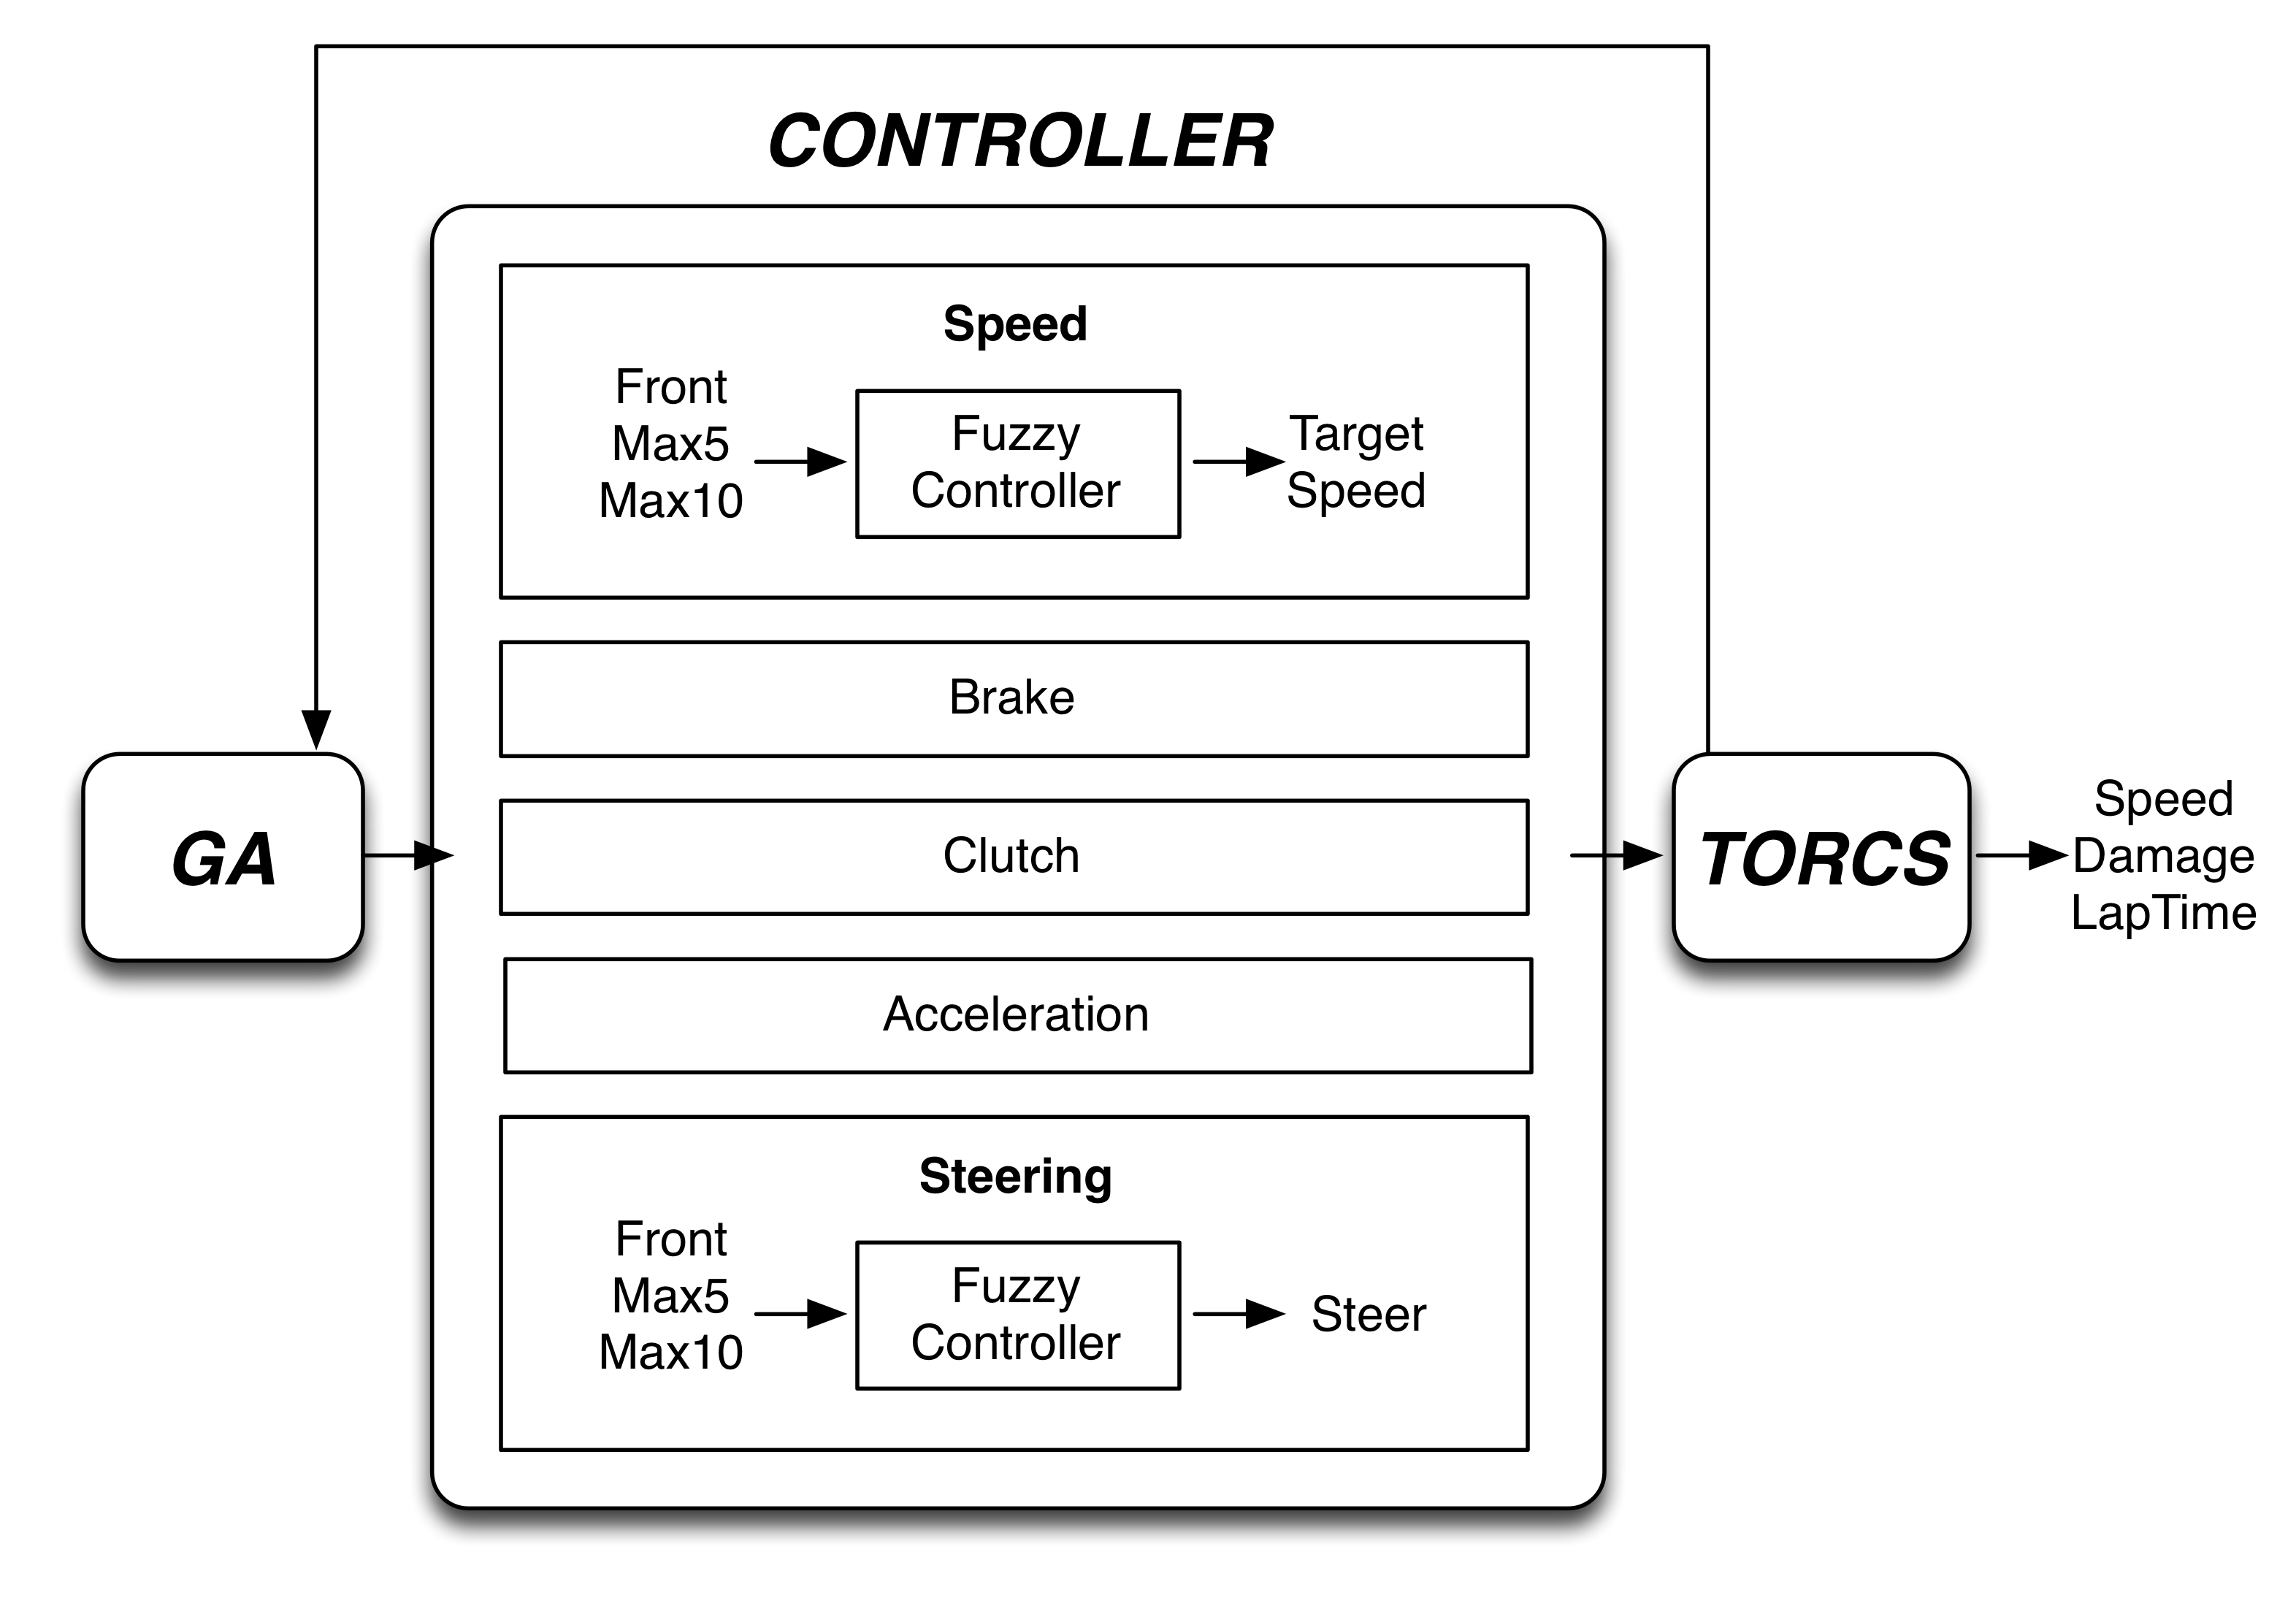
\includegraphics[width=9cm]{fig/flowchart}
  \end{center}
  \caption{Schema of the two controllers that will be evolved by the proposed 
    evolutionary algorithm (GA), and evaluated by TORCS, which will
    return the values for the car's average speed on the complete race and the incurred damage on the vehicle. Figure taken from \cite{salem_evo18}.}
\end{figure}
%
The two fuzzy sub-controllers we evolve take care of target speed and steering angle. These controllers were introduced by the authors in a previous paper \cite{DBLP:conf/evoW/SalemMMG17}, and share the same structure as the standard TORCS driver but they consider five different sensors (see Figure \ref{fig:torcs-sensors}). These controllers are shown in Figure \ref{fig:ga}. 


The \textit{speed controller} takes as input sensor values, and
outputs the target speed; aiming to maximize it straight parts and curves of the circuit. The \textit{steering controller} uses the same sensor values to output the optimal steering angle in order to reach the desired target position with the car.

The two sub-controllers use the same three linguistic variables as
inputs, one for every sensor: one for the frontal sensor,
\texttt{FRONT}, another for Sensors 8 and 10 ($\pm 5$\textdegree),
\texttt{MAX5}, and finally from Sensors 7 and 11 ($\pm
10$\textdegree), \texttt{MAX10}. These variables compose a Mamdani-based fuzzy
system \cite{iancu2012} with three trapezoidal Membership Functions
(MFs) for each variable. The controller uses a set of fuzzy rules
which combine the fuzzy values for these inputs to compute outputs:
target speed or steering angle.
% 
% Antonio - I move this text and tables to the sub-controllers section, since these variables have been defined to be used in the fuzzy rules. Moreover, the variables are introduced for the first time in this section. 
These rules were designed following usual human-like race car driving
rules in \cite{salem_evo18}, are fixed and shown in Table \ref{tab:output}.


\begin{table}[h!tb]
  \centering
  {\scriptsize
    \caption{Rules  \cite{salem_evo18} for speed (top) and steering
      (bottom) controller output. Additionally, when 
      the front, right and left sensors have the maximum value
      possible, a crisp rule that tries to set the max speed
      fires.  Angles will be reversed
      if the M10 is equal to Track 7 in the steering controller. \label{tab:output}}
    \begin{tabular}{|c|c|c||c|}
\hline
      Value Front & Value MAX5 & Value MAX10 & Target Speed (km/h) \\
      \hline
    	 High & - & - & 280 \\
      Medium & - & - & 240 \\
      Low & High & - & 220 \\
      Low & Medium & - & 180 \\
      Low & Low & High & 120 \\
      Low & Low & Medium & 60 \\           
      Low & Low & Low & 30 \\     
\hline
\end{tabular}
\vspace{1em} \\
\begin{tabular}{|c|c|c||c|}
\hline
      Value Front & Value MAX5 & Value MAX10 & $sin$(Steer Angle) \\
\hline
      High & - & - & 0 \\
      Medium & - & High & 0.25 \\
      Medium & Medium & Medium & 0.25 \\
      Medium & Low & Medium & 0.5 \\
      Low & - & High & 0.5 \\
      Low & Medium & Medium & 1 \\
      Low & Low & Medium & 1 \\ 
      
\hline
\end{tabular}
}
\end{table}



Thus, what will be evolved with the algorithm proposed in Section \ref{sec:ga} is the shape of the whole fuzzy system, which is encoded in 18 real-valued parameters (related to the different membership functions). The low-level details of this part was explained extensively in \cite{DBLP:conf/cig/SalemMG19}. 

As mentioned, these fuzzy sub-controllers proved to be a good platform for the evolution of racing car controllers, and have not essentially changed since our first paper. As a matter of fact, the methods presented in this paper could
be applied to any kind of controller, as long as it can be fully
encoded and evolved using an Evolutionary Algorithm (a GA).



%%%%%%%%%%%%%%%%%%%%%%%%%%%%  OPTIMISING WITH GAS  %%%%%%%%%%%%%%%%%%%%%%%%%%%%

\section{Optimizing Sub-controllers with a Genetic Algorithm}
\label{sec:ga}

% Antonio - I think it is more clear if we describe the GA in a separate section, as it is the main contribution of the paper (well, the operators actually, but they would be even more hidden inside a subsection than in a section).

% ------------------- We need to rewrite most of this
% ---------------
% Antonio - I'm going to rewrite this

% -------------------------------------------------------------------
%\subsection{General description}
% You always need to write a description before starting
% subsections. This general description can be it, except we have to
% introduce the other subsections at the end.  
% Antonio - Ok, done.

We have applied a genetic algorithm (GA) \cite{GAs_Goldberg89}, i.e. a type of evolutionary algorithm (EA) \cite{EAs_Back96}, to optimize the parameters of the membership functions of the fuzzy sub-controllers we have been using in this line of research.
% Antonio - I put this text back as we are working with a GA (the title of the section says this), so it is clearer to say what is it. Moreover, the reference is also used in other places, so it is not removed to save space indeed. 
% In addition, there is free available space now. ;)

EAs are nature inspired methods that evolve populations of possible (encoded) solutions for a problem following a process of selection of the best,
recombination and mutation, in order to create a new population of
better individuals on average. This is repeated a number of times
(generations) to get to a solution that meets our requirements, or the
budget we have for evaluation of solutions. EAs have been widely
applied to solve a huge amount of optimization problems, including regression and fuzzy systems \cite{hoffmann2001evolutionary}; in this kind of problem the solutions are modelled as a vector of numeric values, as is the
case in this paper; we use 18 floating-point values, 6 per variable, 2 values per membership function.


% We show in Figure \ref{fig:cromosome} how we represent every individual (chromosome) as a vector of 18 values/parameters (genes), 6 per variable. They have been coded using real values, looking for higher precision \cite{elsayed13}. We started to use this encoding in \cite{10.1007/978-3-319-77538-8_24}.


%  \begin{figure*}[!ht]	
%  	\begin{center}
%  		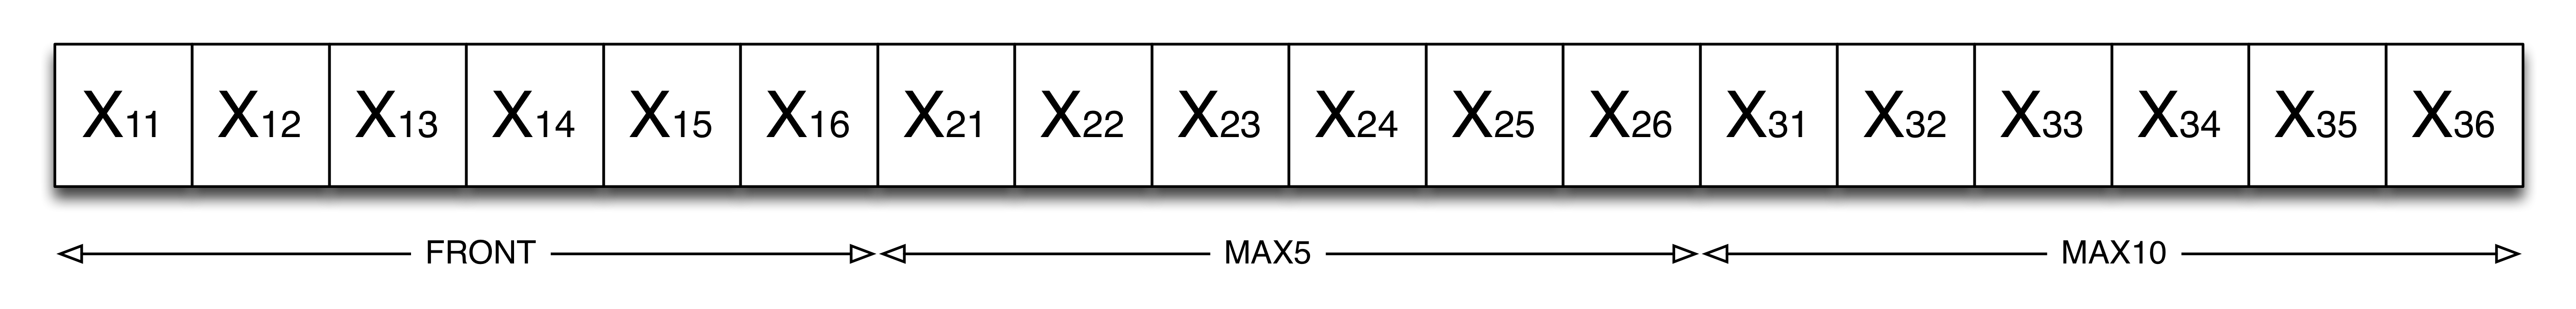
\includegraphics[width=12cm]{fig/chromosome2.png}
%  		\caption{GA chromosome description. There are 6 genes
%                   (values) per fuzzy variable, modelling the 3
%                   different membership functions. The membership
%                   functions are trapezoidal, needing only two values
%                   for every one.}
%  		\label{fig:cromosome}	
%  	\end{center}	
%  \end{figure*}

% \begin{figure*}[!ht]	
% 	\begin{center}
% 		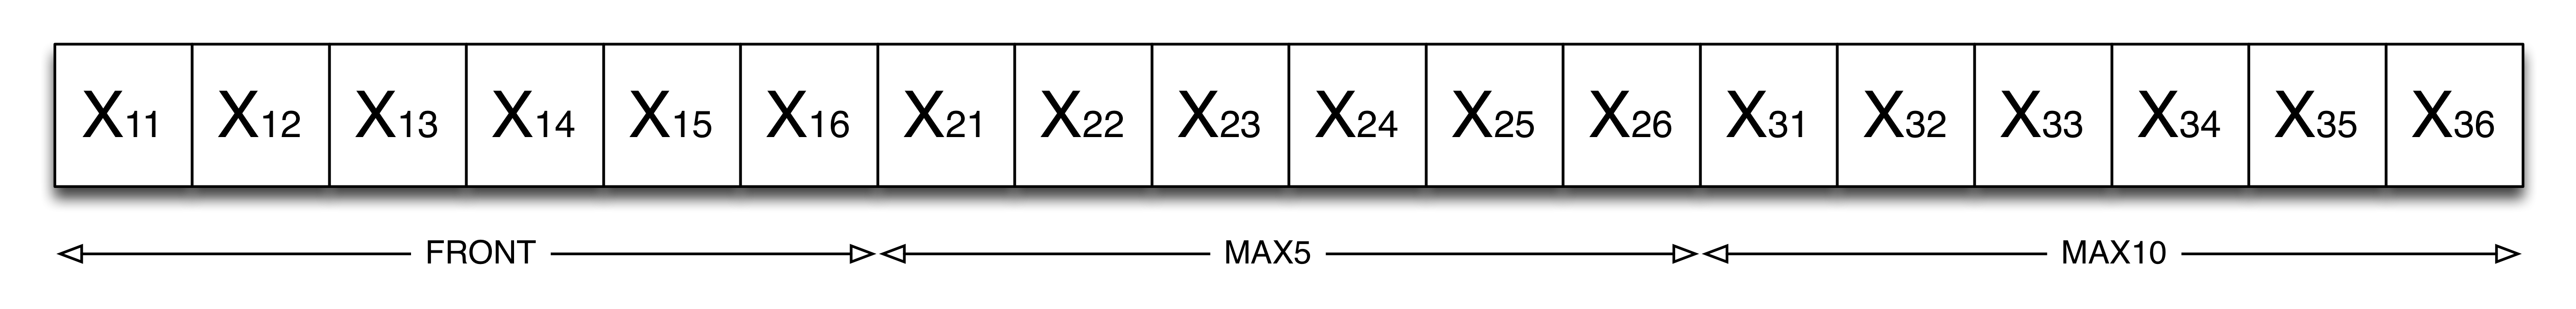
\includegraphics[width=12cm]{fig/chromosome2.png}
% 		\caption{GA chromosome description. There are 6 genes
%                  (values) per fuzzy variable, modelling the 3
%                  different membership functions. The membership
%                  functions are trapezoidal, needing only two values
%                  for every one.}
% 		\label{fig:cromosome}	
% 	\end{center}	
% \end{figure*}



Following standard implementations \cite{GAs_Goldberg89}, in the first step of the algorithm \cite{salem_evo17} a population of random individuals is composed by assigning diverse values inside a feasible range ($[0,100]$).

One of the main factors in EAs is the definition of a function able to determine how good every individual is, this is the \textit{Evaluation Function} or \textbf{Fitness Function}, which must assign the highest value (in maximization problems) to the best individual.
%Mohammed : in maximization problems, not in all cases
% Antonio - right. ;)

As Figure \ref{fig:ga} shows, the evaluation of every individual (controller indeed) is conducted using TORCS. Thus each controller is placed in the simulator, i.e. its gene values are injected to the parameters of the membership functions of the two fuzzy sub-controllers. Then, it competes in several races to evaluate its performance.
Two different approaches have been considered here: one based on a fitness computation and also a fitnessless implementation (that will be explained in Section \ref{subsec:novel_operators}).

The first method considers the fitness function which was defined in a previous work \cite{salem_cig2018}, because it was the most successful among some others proposed \cite{salem_evo18}. It is described in the next equation:

 \begin{equation} \label{fit_avg}
 	\begin{array}{lll}
 		f_{AVS}= \frac{AVG(Speed)}{Damage+1}
 	\end{array}
 \end{equation}	

Where $AVG(Speed)$ is the average speed of the car along the complete race. This factor represents the overall performance of the controller combining difficult (e.g. curves) and easy (e.g. straight) parts of the tracks. $Damage$ value is taken into account in order to preserve the car integrity, which is required to finish the race.

Following the usual recommendations in the literature
\cite{Harik-ParameterLess99}, we have defined a parameterless
selection method, where there are no weights in the terms.
At the same time, this way of evaluating different cars is closer to a `human-like'
approach, since it considers the same prioritary factors that a human
driver would do. 

The evaluation of the individuals (controllers) is done driving a car
in a 20 laps race on a circuit without opponents inside TORCS. The
reason to consider solo-races is to avoid in part the presence of
\textit{noise/uncertainty} due to the participation of other
controllers \cite{merelo2016statistical} in the races. 

\textbf{non uniform mutation} \cite{mutation1997} has been used as the \textit{mutation operator} in the GA, because it was considered in previous approaches of our controllers. 

In the following section we describe two new operators, designed and implemented aiming to improve the algorithm performance, as well as the final quality of the evolved controllers. These are namely a fitnessless selection policy and an extended real-value crossover operator able to manage the balance between exploration and exploitation during the evolution.

% -------------------------------------------------------------------
\subsection{Novel operators}
\label{subsec:novel_operators}

%This paper proposes the inclusion of two different mechanisms into the algorithm in order to improve its performance, as well as they allow to obtain better controllers overall.

The first operator presented is a \textbf{Grand Prix Selection} policy
(GPS), which aims to choose more reliable individuals/controllers as
parents to combine their genes for creating new individuals in the
following generation of the algorithm, as well as use them as a basis
for exploration of new solutions. It is a fitnessless approach,
independent of the aforementioned fitness function (see Equation
\ref{fit_avg}), designed to better deal with the uncertainty present
in the election of an actual good individual. 

The mechanism arranges groups of 10 individuals/controllers which are placed in a track in TORCS, where different races are simulated. Thus, they compete, using the same car (i.e. in the same conditions) during several laps. After every race, the controllers get a score according to their position in the final rank. This is a \textit{score function} based in Formula 1 Grand Prix ranking, so the obtained scores per rank are: rank 1 - 25 points, 2 - 18, 3 - 15, 4 - 12, 5 - 10, 6 - 8, 7 - 6, 8 - 4, 9 - 2, 10 - 1.
Then, the best individuals will be those whose accumulated score (sum of scores of all races) are the five highest.

The objective of this operator is to really select the best individuals of the population. However, given the existing uncertainty \cite{merelo2016statistical} due to the competition against other non-deterministic controllers, it is not possible to ensure they are doubtlessly the best.

In this respect, the authors argue that this operator will provide better individuals than one based on a `standard' fitness function, regarding their competitiveness and reliability. The reasoning for this is the fact that their score just depends on their ability to win the race against other competent controllers, rather than in the combination of a set of variables which might add `noise' to the valuation of the individuals.

However, the application of this method consumes much higher computation time, so it could be combined with a classical fitness-based selection in some generations. Indeed, in the experiments conducted in Section \ref{sec:results}, we have analyzed the impact of the application of different configurations of GPS, considering different frequencies of application during the evolutionary process.

The second operator implemented in our GA is the Blend Crossover or  \textbf{BLX-$\alpha$ Crossover} \cite{blx2008}. As stated before, one of the side effects of uncertainty is the higher diversification factor which it means. Thus, in order to have a better control between the exploration and exploitation factors during the evolution, we have used an \textit{adaptive approach} of the operator.

It is based on the random selection of values from the interval
$[x_i-\alpha(y_i-x_i).. y_i+\alpha(y_i-x_i)]$, where $x_i$ and $y_i$
are the $i^{th}$ parameter values of the parent solutions $x$,$y$ and
$x_i < y_i$. % See Figure \ref{fig:blxalpha}.

% \begin{figure}[!ht]	
%  	\begin{center}
%  		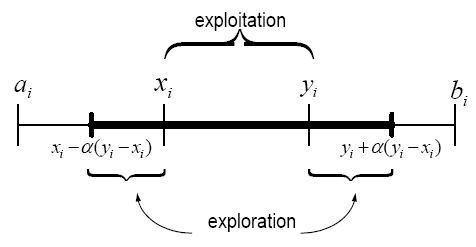
\includegraphics[width=7cm]{fig/blxalpha.jpg}
%  		\caption{Blend crossover operator ($BLX-\alpha$). Figure taken from \cite{Adibo_BLXFig_03}.}
%  		\label{fig:blxalpha}	
%  	\end{center}	
%  \end{figure}
%  Antonio - I include again the figure, because I consider it as very ilustrative to understand how BLX-alpha works. And now we have enough free space.
% It's not the objective of the paper, and it's not even our figure. - JJ

Thus, this crossover method was designed for real-coded EAs \cite{blx2008}, and creates the offspring (i.e. individuals of the new generation) of the current population by selecting random values for every gene around an interval for each of the parents' genes. So, it is able to create three new individuals from one parent, which are different between them and, of course, different to their parent individual. This fact enhances the exploration factor in new generations.

$\alpha$ parameter allows to control the search on the space of solutions, depending on its value, so, a value $\alpha = 0.5$ will establish a balance between exploration and exploitation.

Given the characteristics of an evolutionary algorithm and the way it works, the first generations should be devoted to explore the search space looking for promising areas (those with potential good solutions) where parts of the population could be focused. This would be done by means of a diversification in the individuals. Then, a exploitation process would be recommended, in order to refine the promising solutions to get to an optimal one.

To this end, we have implemented an \textit{adaptive BLX-$\alpha$}
approach, which considers a variable value for $\alpha$. Thus, the
value of this parameter is decreased over the generations, following
the expression: $\alpha =1-\frac{g}{g_{max}}$, where $g$ is the
current generation and $g_{max}$ is the maximum number of generations.

This will mean a higher diversification factor in the first generations, because the offspring will take much more different values for their genes in comparison with their parent and other descendents. %, i.e. the intervals in Figure \ref{fig:blxalpha} will be wider. 
% Antonio - Referencing again Figure. Anyway, the text without this reference was not correct.
On the contrary, as the number of generations is increased, $\alpha$ will take a smaller value, the intervals will be reduced, the individuals will be more similar to their parents, and thus, the space of solutions will be exploited (the solutions will be refined).

We argue that this operator, in conjunction with GPS will aid the algorithm to find better controllers, so we will test several combinations and configurations of both techniques in the experiments conducted in next section. We will also study their impact from different perspectives, both considering their performance and also from the uncertainty influence point of view.


%%%%%%%%%%%%%%%%%%%%%%%%%%%%  RESULTS  %%%%%%%%%%%%%%%%%%%%%%%%%%%%

\section{Experiments and results}  
\label{sec:results}

% >>>>>> TODO: Explain the new experiments and results -> Mohammed  <<<<<<<<<<
% TODO: Results with GPS (no BLX-Alpha crossover)
% TODO: Results with GPS and BLX-Alpha crossover
% TODO: Comparison against the standard controllers in TORCS
% TODO: Comparison against S&PL controller (of all our controllers, if possible)
%
\begin{figure}[!ht]	
	\begin{center}
		
\includegraphics[width=4.5cm]{fig/alpine2.jpg}
		\caption{Alpine 2 Track. Length: 3773.57m, Width: 10m.}
		\label{fig:alpine2_track}	
	\end{center}	
      \end{figure}
%      
In this kind of problems, it is essential to select the correct
training track so that bots are able to work in a wide range of
conditions. Usually a single track, out of all the existing TORCS
ones, is selected, since evaluation in a single track takes some time
and using several of them would make evaluation too onerous. For
several papers already \cite{salem_cig2018,DBLP:conf/cig/SalemMG19},
we have been using the \textit{Alpine 2} track (See Figure
\ref{fig:alpine2_track}). This circuit has several characteristics that
are essential for evaluating a bot: it has got many turns, some of
them with 180 degrees, steep segments, and some very challenging parts
like the entrance of a tunnel at a square angle. All these features make
it a good testbed for good turning and collision avoidance
strategies. Moreover it also offers a few straight segments which allow the car to speed ahead, reaching high speeds. 

This same track has been also repeatedly used by other authors for training as well as for testing and has been described as ``technical and complex'' \cite{AG} and ``presenting a challenge even at low speeds'' \cite{vrajitoru2018global}, for instance in
\cite{cardamone2010applying,CarRacing_Pelta09,zong2017obstacle}; in \cite{AG} it had the third lowest lap time, after Alpine 1 and Olethros, implying it
has got a good balance between hardness and speed. Since we also used
it in our previous papers, it allowed us to compare racing bots that
had been ``trained'' in the same conditions.

Alpine 2 track is probably one of the most popular tracks used for
training; CG-Track 2 has similar features, and it is used by
\cite{mirus2019short,8833873,verma2018programmatically},
in this last case for transfer learning. \cite{Kole-ParamCarTunning12}
mentions CG-Track 2 is "relatively harder", with E-Track 3 the
hardest. On the other hand, \cite{10.1371/journal.pone.0213193} uses
CG-Track 1. There are several differences between CG-Track 2 and Alpine
2, the one we use, but the main one is that turns are relatively
easier and straight segments are longer, favoring fast cars over
balanced ones; this is why we have chosen Alpine 2 for training, since
it offers the best generalization for cars trained using it.

We have again used the vehicle \textit{car1-trb1},
which is a well balanced, NASCAR type car \footnote{See description in
  the TORCS racing board web page,
  \url{http://www.berniw.org/trb/cars/car_view.php?viewcarid=5}},
which we have used also in our previous papers, and also by many
winning bots along the history of the TORCS championship
\cite{torcs5} as well as other authors in the literature
\cite{auteur2010,li2019reinforcement}. This matches well the selection
of racing track, but being as it is a balanced car, allows driving to
fit itself to the controllers we are developing.


%%%%%%%%%%%%%%%%%%%%%%%%%%%%%%%%%%%%%%%%%%%%

To analyze the influence of the new introduced Grand Prix Selection
(GPS) and the crossover operator on the performance of the fuzzy
controller, we have carried out  two main optimization processes based
on the GPS: the first one uses the GPS with the two point crossover
operator while the second uses adaptive BLX-$\alpha$.

For every kind of crossover, three configurations are considered: for
the first one, GPS is applied in every generation giving the new
proposed controllers {\sf GFC-GPSVAE} and {\sf GFC-GPSE}. 
In the second an third configuration, we retrained our previous four  controllers\cite{DBLP:conf/cig/SalemMG19}: {\sf{GFC-GPS5}} and 
{\sf{GFC-GPSVA5}} where GPS selection is used every 5 generation and in the last generation for  {\sf{GFC-GPSL}} and {\sf{GFC-GPSVAL}}.
Also and for comparison purpose, two controllers from previous papers have been considered: {\sf{GFC-VA}}\cite{DBLP:conf/cig/SalemMG19} and {\sf{GFC-VA}}\cite{salem_cig2018}, they both use the fitness function $f_{AVS}$ (Equation \ref{fit_avg}).
All these controllers are summarized in Table \ref{tab:drivers}. 

We have run the algorithms with a population size of 60
individuals. The rest of parameters are: Generations=50, Crossover
rate=0.85, Mutation rate=0.09, and 10 different runs per
configuration. % Clarify if crossover rate means BLX-alpha crossover
               % or there's another crossover too - JJ

We kept the same values for the evolutionary parameters as in our previous works for two reasons: first, because they yielded good results (and are not really the focus of this paper), and second, in order to compare previous controllers with the new ones in the same conditions.


%%%%%%%%%%%%%%%%%%%%%%%%%%%%%%%%%%%%%%%%%%%
\begin{table*}[ht]
	\centering
	{\scriptsize
		\caption{ Description of the controllers tested in the experiments.}
		{
			\begin{tabular}{|c|c|c||c|}
				\hline
				Controller&Fitness & GPS frequency&Crossover operator \\
				\hline
				\hline
{\sf{GFC-GPSE}}&Fitnessless&Every generation&Standard crossover\\
{\sf{GFC-GPSVAE}}&Fitnessless&Every generation&BLX$-\alpha$\\

{\sf{GFC-GPS5}}\cite{DBLP:conf/cig/SalemMG19}&Hybrid&Every 5 generations&Standard crossover\\
{\sf{GFC-GPSVA5}}\cite{DBLP:conf/cig/SalemMG19}&Hybrid&Every 5 generations&BLX$-\alpha$\\

{\sf{GFC-GPSL}}\cite{DBLP:conf/cig/SalemMG19}&Hybrid &Last generation &Standard crossover\\
	
{\sf{GFC-GPSVAL}}\cite{DBLP:conf/cig/SalemMG19}&Hybrid &Last generation&BLX$-\alpha$\\
{\sf{GFC}}\cite{salem_cig2018}& Fitness $f_{AVS}$ (Equation \ref{fit_avg})&-&Standard crossover\\							
{\sf{GFC-VA}}\cite{DBLP:conf/cig/SalemMG19}&Fitness $f_{AVS}$ (Equation \ref{fit_avg})&-&BLX$-\alpha$\\


\hline
				
			\end{tabular}
		}\label{tab:drivers}
	}
\end{table*}
%

% ---------------------------------------------------------------------------

\subsection{Uncertainty in fitness evaluation}

We need first to find out how different kind of selection procedures
affect uncertainty in scores. Better selection procedures should be
able to reduce it, making evolved controllers as centrally distributed
as possible; other kind of selections should keep distribution of
scores (for a single controller) skewed and lopsided; this is why we
have done an study of the distribution  of the genetic individuals of
three evolution processes {\sf GFC}, {\sf GFC-GPSE} and {\sf GFC-GPSVA5}. 


Skewness is related to how symmetric the distribution of fitness
scores is. There are several strategies that deal with this kind of
uncertain (usually called {\em noisy} fitness functions; but a simple
one is to re-evaluate ({\em re-sample}) the score every generation. A
skewed distribution mean that it will more likely to sample a value
that is different from the average, but it might be better or worse
than average; in any case, different from the score we would expect to
achieve in other circumstances. On the other hand, kurtosis measures
the amount of values that are far from the average, creating either a
heavy-tailed or too-lightly-tailed distribution. In the first case, it
will mean that values far from what would be expected are likely to
show up in the fitness score.

This is why we are interested in how these two statistical measures
are going to change with evolution; they will both affect
selectability of an individual, so that, in general, they will select
individuals with lower kurtosis and skewness, since they are more
likely to draw a consistent value and thus go ahead to the next
generation. However, different selection procedures will affect this
in different ways. This is why we have computed skewness and kurtosis for 1 in 5 individuals in the
population chosen randomly, and measured fitness values after the
first, the 20th and the last generation for the three controllers;
results are shown in Figures \ref{fig:gfcsk},\ref{fig:gfcrsesk} and
\ref{fig:gfcvarsesk}). % Which fitness score are we using? - JJ
%% Mohammed $f_{AVS}$ fitness for GFC and GPS for the others

\begin{figure}[!ht]	
	\begin{center}
          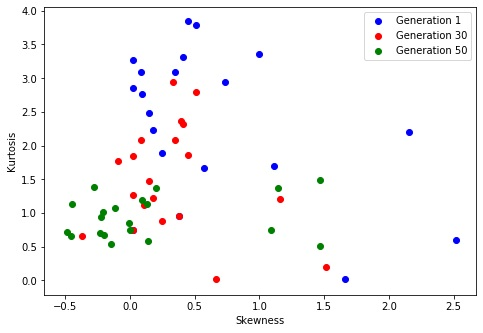
\includegraphics[width=9.5cm]{fig/GFC__.jpg}
          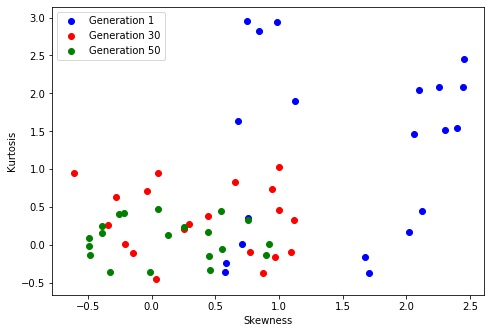
\includegraphics[width=9.5cm]{fig/GFCRSE__.jpg}
          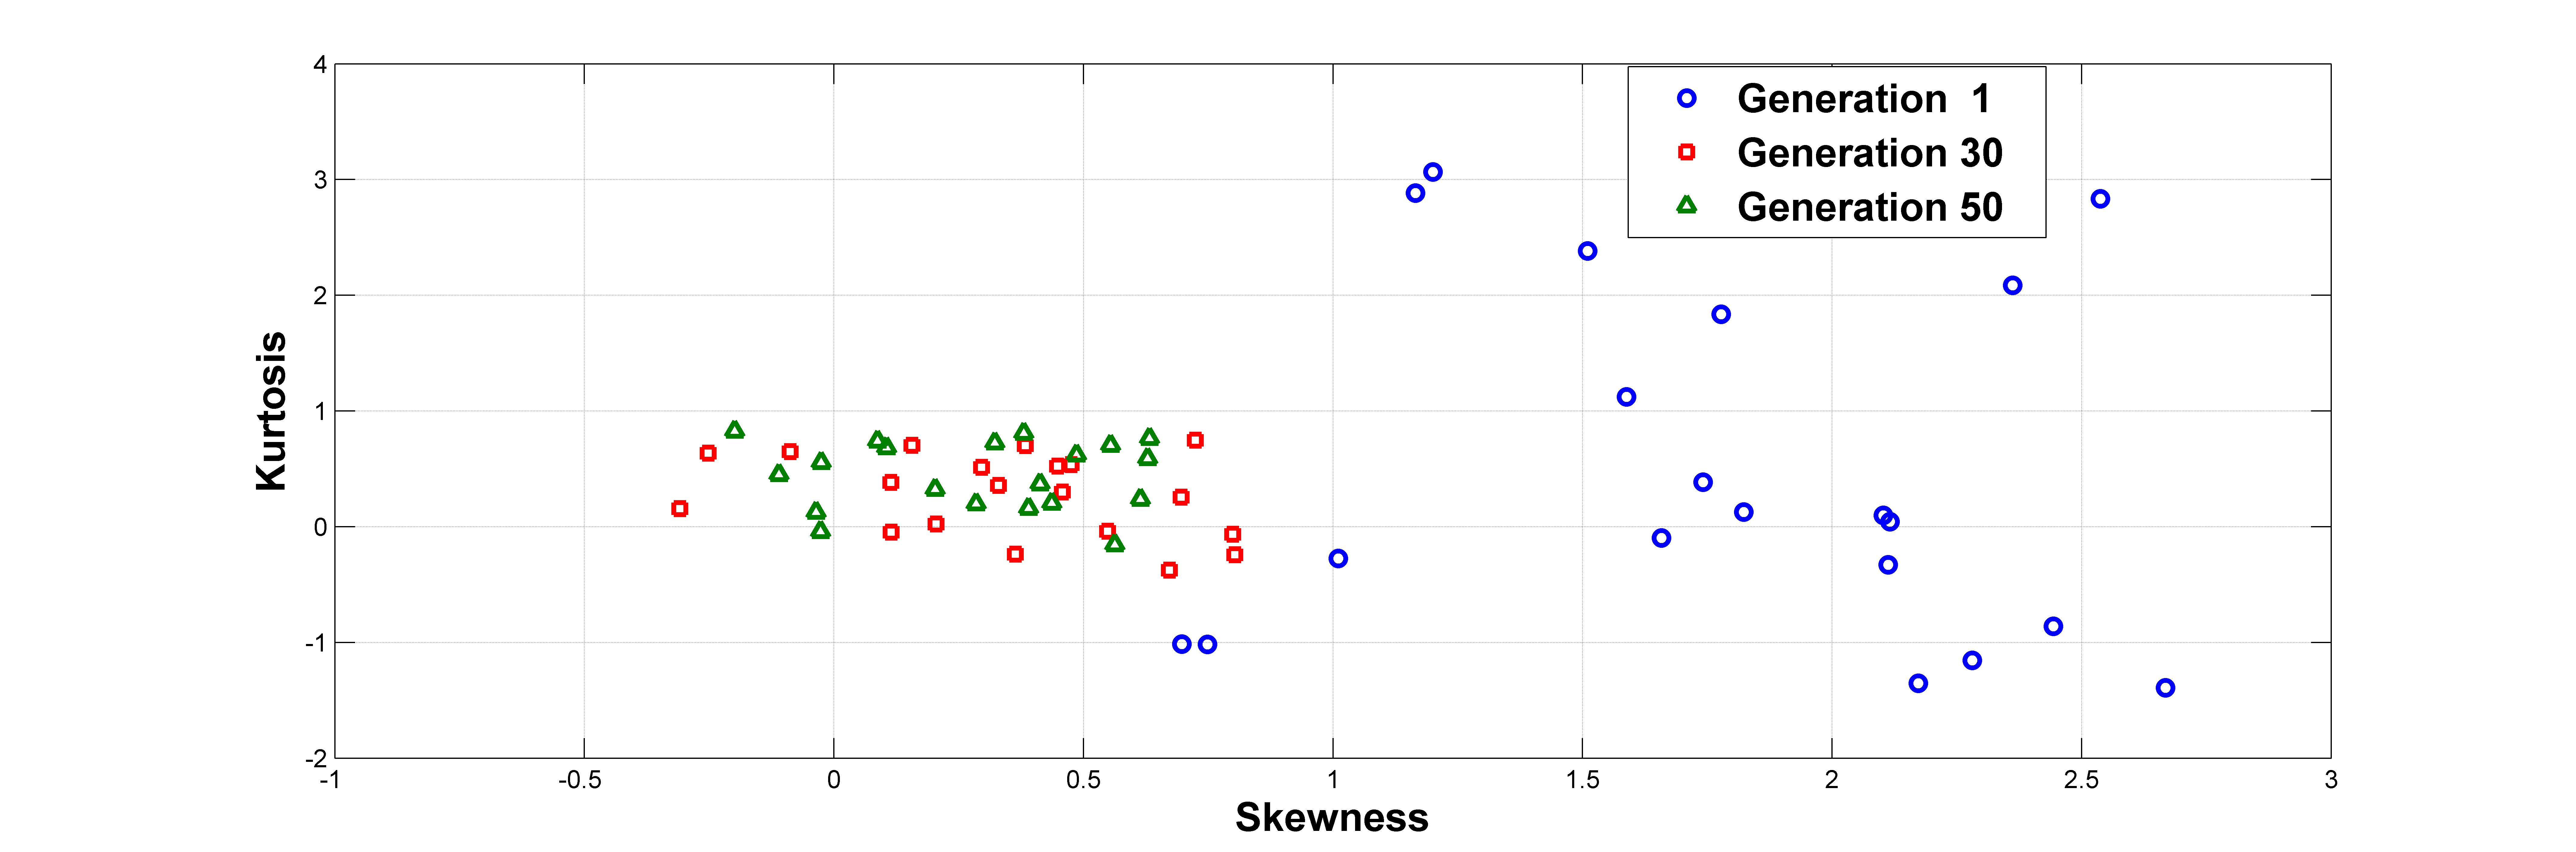
\includegraphics[width=9.5cm]{fig/GFCVARSE__.jpg}
		\caption{Skewness ($y$ axis) and kurtosis ($x$ axis)
                  for the fitness score or chosen individuals in an experiment with the
                  {\sf GFC} method \cite{salem_cig2018} (top), {\sf GFC-GPSE} (middle) and {\sf GFC-GPSVAE} (bottom).}
		\label{fig:gfcsk} \label{fig:gfcrsesk} \label{fig:gfcvarsesk}			
	\end{center}	
\end{figure}

All figures show that the evolution process has a certain influence in
these measures, with individuals in the latest stages of evolution
getting closer to the origin, which would be a 0-skewness, 0-kurtosis
Gaussian. However, there are differences between the fitness-based
process ({\sf GFC}) and the other two. In the first case, the
selection procedure simply eliminates the outliers with a high
skewness or kurtosis; there does not seem to be a big change from
generation 30 to 50, so as a matter of fact individuals with a high
and skewed variability are selected as {\em winners} when in fact they
are not.

The two fitnessless methods, {\sf GFC-GPSE} and {\sf GFC-VA-GPSE}, are
notably similar, with selection eventually concentrating individuals
close to a Gaussian distribution, although slightly skewed to the
right, and with a positive fat tail. However, {\sf GFC-GPSVAE} is able
to find solutions with lower skewness, always between -0.5 and 1,
although kurtosis is slightly higher for the last generation. Since
this method exploits more found solutions, it seems that it is able to
generate new solutions with a more reliable expected value around the
middle of the area the variable covers, but decreasing more slowly
towards values further away from the center. For the time being,
we can affirm that fitnessless methods tend to evolve individuals
with a score that is less uncertain, and thus more robust and whose
expected results are more reliable.

 In the next subsection we
will see how this kind of selection has an influence in the success as
a method for finding high-performance controllers.


% ---------------------------------------------------------------------------

\subsection{Testing Grand Prix selection and BLX-$\alpha$ controllers}


Once the 10 runs have finished, the obtained best controllers from the
previous evolution processes compete again in a similar set of races,
in order to choose the best controller overall per approach, i.e. the
best between {\sf GFC-GPSL}, {\sf GFC-GPSE} and {\sf GFC-GPS5}; and also between
{\sf GFC-GPSVAL}, {\sf GFC-GPSVAE} and {\sf GFC-GPSVA5}. 
Results are shown in Tables\ref{tab:RSresults} and \ref{tab:VaryingalphaRSresults}
%% Process 1 : GPS without Alpha
%% Process 2  : GPS with Alpha
%%  GFC and VA are used only in comparaison purpose

\begin{table}[ht]
	\centering
	{\scriptsize
		\caption{ Results of controllers using GPS in a mini-championship with 10 controllers and 10
			races in two different tracks(20 laps each). {\tt tita}, {\tt berniw} and {\tt
				inferno} are example controllers included with the TORCS
			simulator \cite{torcs4}. We use {\bf boldface}
                      for the best value, {\em italics} for the second
                    best. }
		{
                  \begin{tabular}{|c|c|c||c|}
                    \hline
                    & \multicolumn{2}{|c|}{Score in} & \\
                    \hline
                    Controller&\textit{Alpine 2} track &\textit{E-Track 5} track &Total\\
				\hline
				\hline
				
			{\sf GFC-GPS5}\cite{DBLP:conf/cig/SalemMG19}&	75	&74&	149\\
			{\sf GFC-GPSE}&	98	&93&	{\bf 191}\\
			{\sf GFC-GPSL}\cite{DBLP:conf/cig/SalemMG19}&	77	&81&	{\em 158}\\
			{\sf GFC} \cite{salem_cig2018}	&	56	&50&	106\\
			{\sf GFC-VA}\cite{DBLP:conf/cig/SalemMG19}	&	46	&7&		53\\
			$inferno1$&	9	&8&		17\\
			$inferno2$&		20	&51&	71\\
			$berniw1$&	16	&24&	40\\
			$berniw2$&	76	&79&	155\\
			$tita1$&32	&38&	70\\		
				\hline
				
			\end{tabular}
		}\label{tab:RSresults}
	}
\end{table}
%


%
\begin{table}[ht]
	\centering
	{\scriptsize
          \caption{ Results of {\sf GFC-GPSVAE} controllers in a mini-championship with 10 controllers and 10
            races in two different tracks(20 laps each). {\tt tita}, {\tt berniw} and {\tt
              inferno} are example controllers included with the TORCS
            simulator \cite{torcs4}. {\bf Boldface}
            for the absolute winner, {\em italics} for the second
            best.}
          {
            \begin{tabular}{|c|c|c||c|}
              \hline
              & \multicolumn{2}{|c|}{Score in} & \\
              \hline
              Controller& \textit{Alpine 2} track & \textit{E-Track 5} track &Total\\
              \hline
              \hline	
              {\sf GFC-GPSVA5} \cite{DBLP:conf/cig/SalemMG19}&	82&	82&	{\em 164}\\
              {\sf GFC-GPSVAE} &	108&    101&	{\bf 209}\\
				{\sf GFC-GPSVAL} \cite{DBLP:conf/cig/SalemMG19}&	77&	73&	150\\
				{\sf GFC}  \cite{salem_cig2018}&	56&	50&	106\\
				{\sf GFC-VA} \cite{DBLP:conf/cig/SalemMG19}&	46&	7&	53\\
				$inferno1$&	9&	8&	17\\
				$inferno2$&	20&	49&	69\\
				$berniw1$&	16&	24&	40\\
				$berniw2$&	59&	73&	132\\
				$tita1$&	32&	38&	70\\			
				\hline
				
			\end{tabular}
		}\label{tab:VaryingalphaRSresults}
	}
\end{table}
%
As it could be noticed in the Table \ref{tab:RSresults}, the controller {\sf GFC-GPSVAE} has win the Grand Prix championship obtaining 98 points from 125 in the track used in the training, it has also ranked first in the track  \textit{E-Track 5}. //
The other GPS based controllers have obtained nearly the same results (149 and 158 respectively).
From Table \ref{tab:RSresults},it is clear that the controller {\sf GFC-GPSVAE}, where GPS selection has been applied in every generation, has won the majority of possible points in the two previous tracks even the unknown \textit{E-Track 5}  track.

These results come to confirm the influence of the proposed selection policy where the controllers obtained from applying the GPS selection alone have won the competition.
 
This results is evident when comparing the points obtained by GPS controllers and GFC.
Indeed, we have made the selection process  realistic by eliminating
the classical fitness function based on the speed and damage average
and replacing it by points obtained in direct races. 
Better speed in solo racing is not a criterion of a good controller, the
best is the one who wins races. The new selection policy allows you to
select the winners on the field and not the possible winners. 
The following experimentation is dedicated to detect the impact of the $BLX-\alpha$.
The best controllers obtained from the two main optimization
processes: {\sf GFC-GPSVAE} and {\sf GFC-GPSE} are evaluated in formula like
championship against the references five TORCS bots and the {\sf GFC-VA}\cite{DBLP:conf/cig/SalemMG19}
and {\sf GFC} controllers  \cite{salem_cig2018}. We have considered also an opponent from the
state of the art, which participated in several Simulated Car Racing
Competitions in past editions.  % Rewrite this paragraph too, from "We
                                % have considered" - JJ
It was proposed by P{\'e}rez-Li{\'e}bana, S{\'a}ez, Recio and Isasi
\cite{EvolvingRuleSystem08} and later refined in the work
\cite{PerezEvolvingFuzzy09}. We have baptized it as PSRI in honor of
its authors' surnames; results in Table \ref{tab:allsresults}.
%
\begin{table}[ht]
  \centering
  {\scriptsize
    \caption{ Results of {\sf GFC-GPSVAE} and {\sf GFC-GPSE}
      controller in a mini-championship with 10 controllers
      and 10 % you use driver here, controller
      % elsewhere. Use always one or the other - JJ
      %% mOhammed ok 
      races in two different tracks(20 laps each). {\tt tita}, {\tt berniw} and {\tt
        inferno} are example controllers included with the TORCS
      simulator \cite{torcs4}.  {\bf Boldface} is
      used to highlight the best value, {\em italics} for the second
      best.}
    {
      \begin{tabular}{|c|c|c||c|}
        \hline
        & \multicolumn{2}{|c|}{Score in} & \\
        \hline
        Controller&\textit{Alpine 2} track &\textit{E-Track 5} track &Total\\
        \hline
        \hline
{\sf GFC-GPSE}&	85&	82&	{\em 167}\\
{\sf GFC-GPSVAE}&111&101&            {\bf 212}\\
{\sf GFC}  \cite{salem_cig2018}&		48&	55&	103\\
$PSRI$\cite{PerezEvolvingFuzzy09}&		53&	48&	101\\
{\sf GFC-VA} \cite{DBLP:conf/cig/SalemMG19}&	78&	64&	142\\
$inferno1$&	9&	8&	17\\
$inferno2$&	20&	40&	60\\
$berniw1$&	16&	24&	40\\
$berniw2$&	59&	69&	128\\
$tita1$&	26&	18&	44\\
					\hline
				
			\end{tabular}
		}\label{tab:allsresults}
	}
\end{table}
%



The above competition clearly demonstrates the superiority of the {\sf GFC-GPSVAE} controller where it clearly leads in the points. It collected most of the points in the two tracks, leaving the {\sf GFC-GPSE} controller far behind it. The reference conductors, namely {\sf GFC-VA} and {\sf GFC}  are classified 3rd and 5th.
The introduction of the $BLX-\alpha$ operator allows the parameters of the controllers to be refined and  increases diversification in the optimization process, which has led to better results than those of {\sf GFC-GPSE}.

%%%%%%%%%%Add  controller GFC-VAGPSE MFs
The structure of the winner controller {\sf GFC-GPSVAE} is depicted in Figure \ref{fig:frontmfs}. % Some comments are needed.

\begin{figure}[!ht]	
  \begin{center}
    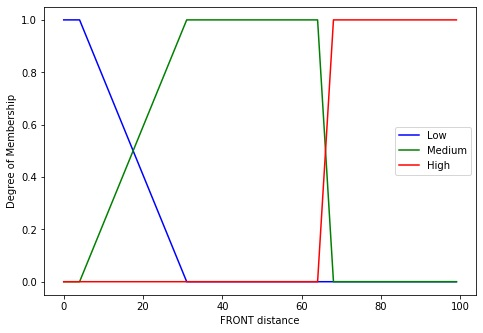
\includegraphics[width=9cm]{fig/FRONT.jpg}
    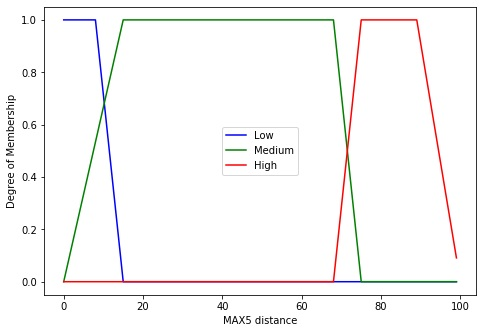
\includegraphics[width=9cm]{fig/MAX5.jpg}
    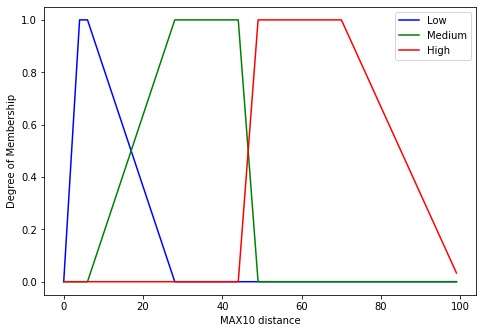
\includegraphics[width=9cm]{fig/MAX10.jpg}		
    \caption{Front, Max5 and Max10 input membership functions for a controller obtained with the 
      {\sf GFC-GPSVAE} method.}
    \label{fig:frontmfs}
    % Is this the steering or the speed controller? We will need to publish both - JJ
  \end{center}	
\end{figure}
%\begin{figure}[!ht]	
%	\begin{center}
%		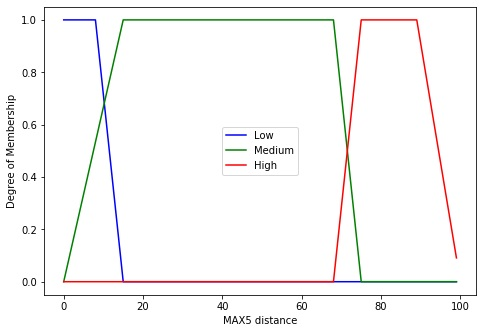
\includegraphics[width=9cm]{fig/MAX5.jpg}
%		\caption{MAX5 input membership for 
%			{\sf GFC-GPSVAE}.}
%		\label{fig:max5mfs}	
%	\end{center}	
%\end{figure}
%\begin{figure}[!ht]	
%	\begin{center}
%		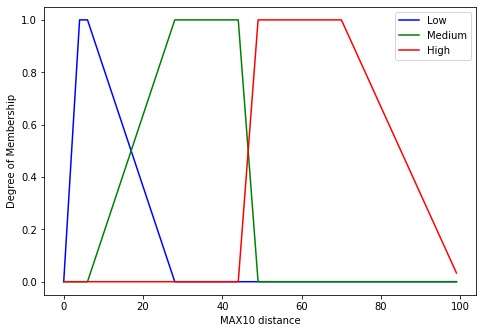
\includegraphics[width=9cm]{fig/MAX10.jpg}
%		\caption{MAX10 input membership for 
%			{\sf GFC-GPSVAE}.}
%		\label{fig:max10mfs}	
%	\end{center}	
%\end{figure}


If we take into account the rules already set in Table \ref{}, the shape of the obtained MFs  is in accordance with what a human driver would have done: favor speed as much as possible in the straight sections and brake as late as possible in the turns.
According to the figures, we have more than three quarters of probability that the first three rules will activate, these rules would make the car very aggressive especially in the straight sections of the track.
%%%%%%%%%%%%%%%%%%%%%%%%%%%%%%%%%%%%%%%%%%%%%%

To evaluate the cost of the proposed controllers, the table \ref{tab:time} shows the average number of laps % Isn't this
% average running time? - JJ
%% each lap in Alpine 2  takes between 90s and 120s
%%  I prefered the laps number to high time values ( 123800s for instance) 
and the range of the generation where the best individual is found of all the considered controllers. These results are obtained by running genetic
optimization for 50 generations for 10 runs.  

\begin{table}[!ht]
	\centering
	{\scriptsize
          \caption{Average runtime (s) in 10 runs
          	 %  Isn't this
                                %  average running time? - JJ
            and
                  generation where the best individual was spawned.}
		\label{tab:time}
		\begin{tabular}{|p{2.85cm}|p{2cm}|p{1.65cm}|}
			\hline  
			Controller& \textbf{Average Runtime}&\textbf{Generation}\\
% Is this number of laps or running time? - Jj
%Mohammed %% each lap in Alpine 2  takes between 90s and 120s
%% number of completed laps,  I prefered the laps number to high
%% values of average running time values ( 123800s for instance)
                  % But still all cars run the same amount of laps in
                  % every race. It probably makes sense to use time
                  % here - JJ
                  \hline
                  			\hline 	 \textbf{\textbf{{\sf GFC}}} \cite{salem_cig2018}&294000
                   &34-39\\
\textbf{{\sf GFC-VA}} \cite{DBLP:conf/cig/SalemMG19}&279000
			 	&10-18\\	
 \textbf{{\sf GFC-GPSL}} \cite{DBLP:conf/cig/SalemMG19}& 282945
			 &23-38\\	
 \textbf{{\sf GFC-GPS5}} \cite{DBLP:conf/cig/SalemMG19}&331320
				&24-38\\	
 \textbf{{\sf GFC-GPSE}}&	276600
			 &22-40\\	
 \textbf{{\sf GFC-GPSVAL}} \cite{DBLP:conf/cig/SalemMG19}& 270923
				&9-15\\	
\textbf{{\sf GFC-GPSVA5}} \cite{DBLP:conf/cig/SalemMG19}&	326520
			 &8-17\\	
\textbf{{\sf GFC-GPSVAE}}& 273000
				&11-18\\					
			\hline 
		\end{tabular}
		
	}
\end{table} 

The two {\sf GFC-GPSVAE} and {\sf GFC-GPSE} controllers were the best where
they are ranked $1^st$ and $2^nd$ but they are very expensive in runtime
where they have performed around 273000s and 276600s respectively, which is a
huge learning time. % Don't all individuals use the same amount of
                    % laps to race? - JJ
                    
                 % Mohammed : in fitnessless  case , time of a race is the time of the worst individual 
                 % Time of BLX based aproaches, ind are close to each other, so the difference between the best and the wort is less, this factor, decreases the whole runtime
                 
The proposed selection policy is effective but in return it requires a
lot of time.%% this drawback was reduced using parallel computing. % We
                                % used parallel computing?? -- JJ
%
Another point that we can highlight is that the controllers with
$BLX-\alpha$ have reached the optimal solution in few generations
(between the $10^th$ and the $20^th$) while the other methods required more
generations. 


 %%%%%%%%%%%%%%%%%%%%%%%%%%%%
\section{Conclusions and Future Work} 
\label{sec:conclusions}

% >>>>>> TODO: Rewrite this section -> All  <<<<<<<<<<
In this paper, and in order to avoid the impedance between using solo
racing scores and performance in competitive races, we hace
incorporated this competition into the selection of individuals in an
evolutionary algorithm that evolves fuzzy controllers in the TORCS
game, and evaluated it in combination with hybrid methods that use
that selection only part of the time, and an adaptive BlX-$\alpha$ and
a normal crossover algorithm, to assess how it interacts with them and
which combination yields the best competitive results.

% Rewritten above --- ^^^ ---
% This paper is dedicated to present a new selection policy to replace
% the use of standard fitness in genetic algorithms that optimize a
% fuzzy controller for racing cars in the TORCS simulator. The
% performance of this type of algorithm fully depends on the choice of
% the appropriate fitness function and on certain operators’ parameters
% such as crossover and mutation. Furthermore, in car racing, we have an
% additional difficulty which is the uncertainty caused by opponents
% decisions and track state where we would be forced to handle
% non-deterministic fitness values. 

% -------------------- this is reiterative and does not add anything -----
% We tried in a previous work to design a fitness which eliminates this uncertainty or reduces it by looking for the parameters which most affect the behavior of the controllers but the results obtained were not sufficiently satisfactory. In this paper, we started from a simple hypothesis: what if we let nature make the selection? Indeed, since the objective is to find the parameters of a winning controller, why not get rid of fitness and let nature do the rest.
% The main idea of this work is to overcome uncertainty by using a
% selection policy based on a system similar to Grand Prix championships
% where the score of a controller is the sum of the points collected
% during a set of races and in order to speed up the optimization
% process, we have introduced a new crossover operator: BLX-$\alpha$
% which improves exploration.
% ----------------------------------------------------------------

% --------------- this is just a repetition of results, not a
% conclusion --- 
% A statistical study has led us to affirm that the proposal makes it
% possible to face uncertainty thus giving a robust and reliable
% controller and the introduction of the operator BLX-$\alpha$ has
% allowed a clear acceleration of the process of genetic optimization
% while the comparison of the optimized controller with other ones from
% the literature has shown the robustness of the fuzzy controller where
% it has won the majority of races being the first in the general
% ranking.

In races performed in the training, and other, tracks, the controller
that has evolved using competitive (fitness-less) selection and the
variable $\alpha$ BLX crossover operator has proved superior to not
only other controllers evolved previously by us, but also other
competitive entries. As a matter of fact, using GPS has the greatest 
influence in the results: {\sf GPSVAE} and {\sf GPSE}, whose only
difference lies in the kind of crossover operator they use, create the
best controllers, finishing first and second in competitive races and,
in the first case, obtain twice the score of the non-evolved
competitor, $berniw2$. The variable-$\alpha$ BLX operator seems to
have also a positive influence in the outcome, outperforming the fixed
BLX-$\alpha$ in a race, as shown in the competitive races presented in
this paper. The decreasing amount of exploration that adaptive
BLX-$\alpha$ boasts explores in a more efficient way the space of
controllers, finding very competitive solutions.

Another advantage of these combined methods is that they don't
increase total training time, and are also able to find a good
solution in the first stages of evolution, which, if needed, allows to
cut the training short. {\sf GFC-GPSVAE} needs at most 18 generations
(which is around one third of the maximum number of generations) to
find a good solution. Running GPS every generation needs more
genrations that if it's run every 5 generations, or just at the end,
but the problem is that in those cases the solution found is less
competitive. However, {\sf GPS-VA5} is quite competitive, and in the
case of a limited evaluation budget, it could be a very good
compromise.

As a conclusion, in this paper we have proved that combining a
fitness-less evolutionary algorithm with an adaptive, floating point,
crossover operator, consistently obtains the best results so far in
TORCS. The sets of choices of running track, car, controller and
actually parts of it that are evolving are thus also validated by
these results.

However, results are probably independent of the fact that we are using a
set of fuzzy controllers. The result could be generalized to any kind
of controllers, as long as they have the possibility to explore the
space of controllers in the same, efficient, way. This is a possible
way of extending the work: substituting fuzzy controllers by simple
neural nets could be a way of proving that the fitness-less approach
is able to find good results independently of the low-level algorithms
using to drive the car. Fuzzy and neural controllers could be also
mixed, even coevolved, to try and find the best ones. 

Additionally, we have been using heuristic rules for computing outputs
from the fuzzy rule activation. We could, however, consider optimizing
the outputs of the fuzzy controllers, as well as the rules.

The implementation could also be optimized. Right now, training takes
a long time. This optimization could go from parallelization, to basic
program-level improvement. All this is left as future work.



\section*{Acknowledgments}

This work has been supported in part by: Ministerio espa\~{n}ol de
Econom\'{\i}a y Competitividad under projects  TIN2017-85727-C4-2-P (UGR-DeepBio) and TEC2015-68752 (also funded by FEDER), as well as project RTI2018-102002-A-I00 (Ministerio espa\~{n}ol de Ciencia, Innovaci\'{\o}n y Universidades).

\bibliographystyle{IEEEtranS}
\bibliography{fuzzy_torcs,geneura,uncertainty,fitnessless}


% Antonio - This should be included once it is accepted
%\begin{IEEEbiographynophoto}{Juan~J.~Merelo}
%Biography text here.
%\end{IEEEbiographynophoto}


% You can push biographies down or up by placing
% a \vfill before or after them. The appropriate
% use of \vfill depends on what kind of text is
% on the last page and whether or not the columns
% are being equalized.

%\vfill

% Can be used to pull up biographies so that the bottom of the last one
% is flush with the other column.
%\enlargethispage{-5in}



% that's all folks
\end{document}
